%\documentclass[amsmath,table,sans,amsfonts, handout]{beamer}
\documentclass[amsmath,table,sans,amsfonts]{beamer}
\usepackage[T1]{fontenc}
%%\usepackage{beamerthemeshadow}
%%\usepackage[headheight=1pt,footheight=10pt]{beamerthemeboxes}
%%\addfootboxtemplate{\color{structure!80}}{\color{white}\tiny \hfill Karl Svozil (TU Vienna)\hfill}
%%\addfootboxtemplate{\color{structure!65}}{\color{white}\tiny \hfill mur.sat \hfill}
%%\addfootboxtemplate{\color{structure!50}}{\color{white}\tiny \hfill Graz, 2010-12-11\hfill}
%\usepackage[dark]{beamerthemesidebar}
%\usepackage[headheight=24pt,footheight=12pt]{beamerthemesplit}
%\usepackage{beamerthemesplit}
%\usepackage[bar]{beamerthemetree}
\usepackage{graphicx}

%Global Background must be put in preamble
{%
%\usebackgroundtemplate%      \includegraphics[width=\paperwidth,height=\paperheight]{HaK-Urkaos-da}%
}
 \setbeamercolor{background canvas}{bg=black}

%\usepackage{eepic}
%\usepackage[usenames]{color}
%\newcommand{\Red}{\color{Red}}  %(VERY-Approx.PANTONE-RED)
%\newcommand{\Green}{\color{Green}}  %(VERY-Approx.PANTONE-GREEN)


%\RequirePackage[german]{babel}
%\selectlanguage{german}
%\RequirePackage[isolatin]{inputenc}

%\pgfdeclareimage[height=0.5cm]{logo}{tu-logo}
%\logo{\pgfuseimage{logo}}
\beamertemplatetriangleitem
%\beamertemplateballitem

\beamerboxesdeclarecolorscheme{alert}{red}{red!15!averagebackgroundcolor}
%\begin{beamerboxesrounded}[scheme=alert,shadow=true]{}
%\end{beamerboxesrounded}

%\beamersetaveragebackground{yellow!10}

%\beamertemplatecircleminiframe

\newtheorem{question}{Question}
\newtheorem{conjecture}[question]{Principle}
\newtheorem{challenge}[question]{Challenge}

\usepackage{tikz}
\usetikzlibrary{decorations.pathreplacing,decorations.markings}





        \definecolor{orange(webcolor)}{rgb}{1.0, 0.65, 0.0}
\setbeamercolor{normal text}{fg=yellow}
\setbeamercolor{structure}{fg=yellow}




\begin{document}




\title{\bf \textcolor{orange!100}{Breathing in and out of Entanglement}}
\subtitle{\textcolor{orange!100}{\small http://tph.tuwien.ac.at/$\sim$svozil/publ/2017-Svozil-WOE-pres.pdf
%\\
%Nature-Springer, in press 2017; drafts on demand
}}
\author{\textcolor{orange!100}{Karl Svozil}}
\institute{\textcolor{orange!100}{ITP/Vienna University of Technology, Austria\\
\& CS/University of Auckland, NZ  \\
svozil@tuwien.ac.at
}
%{\tiny Disclaimer: Die hier vertretenen Meinungen des Autors verstehen sich als Diskussionsbeitr�ge und decken sich nicht notwendigerweise mit den Positionen der Technischen Universit�t Wien oder deren Vertreter.}
}
\date{\textcolor{orange!100}{Brussels, Belgium, EU, Sept 30th, 2017}}

\maketitle

% \frame{
% \frametitle{}
%
% }




 \frame{
 \frametitle{Questions one could ask}

\begin{itemize}
%\pause
\item
What is entaglement?

\item
How can entaglement be produced?

\item
How can a state ``breathe in \& out of entanglement?''

\item
What is the connection between entanglement \& ``non-locality?''

\item
Has entanglement a role in measurement?


\end{itemize}



 }






\frame{
\frametitle{How it all started:
Schr\"odinger on individuation,  entanglement and qm object-observer relation}



Schr\"odinger again (cat papers, 1935) wrt entanglement and individuality:
{\em ``The whole is in a definite state, the parts taken individually are not.''}

German original: {\em ``Das Ganze ist in einem bestimmten Zustand,
die Teile f\"ur sich genommen nicht.''}

\begin{center}
{\color{orange}
$\widetilde{\qquad \qquad }$
$\widetilde{\qquad \qquad}$
$\widetilde{\qquad \qquad }$
}
\end{center}

Bennett:
 {\em ``that you have a complete knowledge
of the whole without knowing the state of any one part. That a thing can be in a definite
state, even though its parts were not.~$\ldots$
It's not a complicated idea but
it's an idea that nobody would ever think of.''}

https://youtu.be/9q-qoeqVVD0





}

\begin{frame}[fragile]{Possible production scheme}

Is entanglement nothing but the manifestation of coherent superpositions among (classically mutually exclusive)
multipartite states? Eg, Bell basis:

\begin{center}
%\includegraphics[width=8cm,angle=0]{2017-etpi-f1.png}

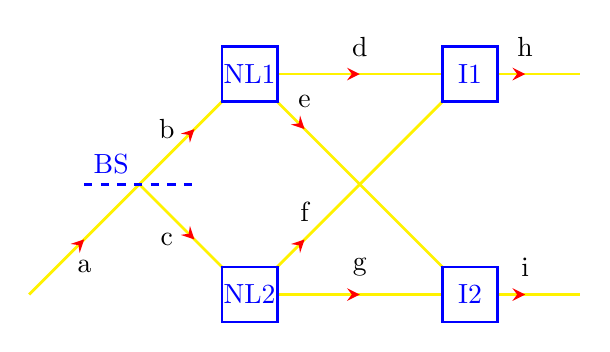
\begin{tikzpicture} [scale=1.4]

\tikzstyle{every path}=[line width=1pt ]

\tikzset{
  % style to apply some styles to each segment of a path
  on each segment/.style={
    decorate,
    decoration={
      show path construction,
      moveto code={},
      lineto code={
        \path [#1]
        (\tikzinputsegmentfirst) -- (\tikzinputsegmentlast);
      },
      curveto code={
        \path [#1] (\tikzinputsegmentfirst)
        .. controls
        (\tikzinputsegmentsupporta) and (\tikzinputsegmentsupportb)
        ..
        (\tikzinputsegmentlast);
      },
      closepath code={
        \path [#1]
        (\tikzinputsegmentfirst) -- (\tikzinputsegmentlast);
      },
    },
  },
  % style to add an arrow in the middle of a path
  mid arrow/.style={postaction={decorate,decoration={
        markings,
        mark=at position .5 with {\arrow[#1]{stealth}}
      }}},
 % style to add an arrow in 1/4th of a path
  onefourth arrow/.style={postaction={decorate,decoration={
        markings,
        mark=at position .25 with {\arrow[#1]{stealth}}
      }}},
}

 \path
  (0,0) coordinate(1)
  (1,1) coordinate(2)  % BS
  (2,2) coordinate(3)  % NL1
  (2,0) coordinate(4)  % NL2
  (4,2) coordinate(5)  % I1
  (4,0) coordinate(6)  % I2
  (5,2) coordinate(7)  % h
  (5,0) coordinate(8)  % i
  (0.5,1) coordinate(9)  % BSa
  (1.5,1) coordinate(10)  % BSb
;


\path [draw=yellow,postaction={on each segment={mid arrow=red}}]  (1) -- (2) -- (3);
\path [draw=yellow,postaction={on each segment={mid arrow=red}}]  (2) -- (4);
\path [draw=yellow,postaction={on each segment={mid arrow=red}}]  (3) -- (5);
\path [draw=yellow,postaction={on each segment={onefourth arrow=red}}]  (3) -- (6);
\path [draw=yellow,postaction={on each segment={onefourth arrow=red}}]  (4) -- (5);
\path [draw=yellow,postaction={on each segment={mid arrow=red}}]  (4) -- (6);
\path [draw=yellow,postaction={on each segment={mid arrow=red}}]  (6) -- (8);
\path [draw=yellow,postaction={on each segment={mid arrow=red}}]  (5) -- (7);
\path [draw=blue,dashed]  (9) -- (10);
\draw [blue,fill=white] (3) ++(-0.25,-0.25) rectangle node {NL1} ++(0.5,0.5);
\draw [blue,fill=white] (4) ++(-0.25,-0.25) rectangle node {NL2} ++(0.5,0.5);
\draw [blue,fill=white] (5) ++(-0.25,-0.25) rectangle node {I1} ++(0.5,0.5);
\draw [blue,fill=white] (6) ++(-0.25,-0.25) rectangle node {I2} ++(0.5,0.5);
\draw [blue] (2) coordinate[label=100:BS];

\node (a) at (0.5,0.25) {a};
\node (b) at (1.25,1.5) {b};
\node (c) at (1.25,0.5) {c};
\node (g) at (3,0.25) {g};
\node (d) at (3,2.25) {d};
\node (e) at (2.5,1.75) {e};
\node (f) at (2.5,0.75) {f};
\node (h) at (4.5,2.25) {h};
\node (i) at (4.5,0.25) {i};

\end{tikzpicture}
\end{center}

\end{frame}

\begin{frame}[fragile]{Possible production scheme cntd.}

\begin{center}
%\includegraphics[width=8cm,angle=0]{2017-etpi-f2.png}
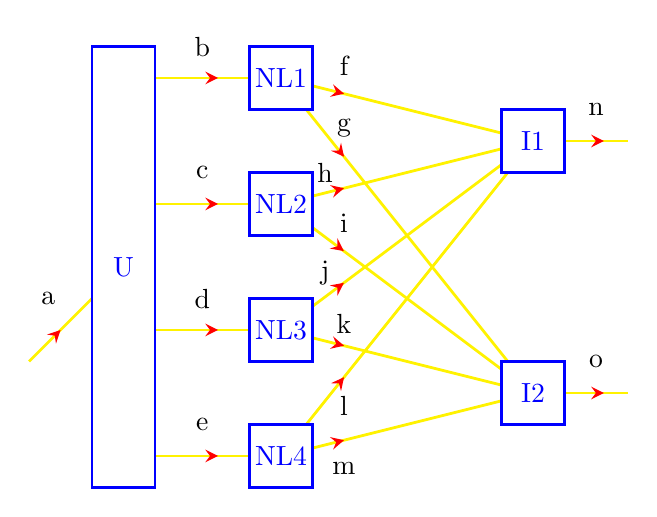
\begin{tikzpicture} [scale=0.8]

\tikzstyle{every path}=[line width=1pt]
\tikzset{
  % style to apply some styles to each segment of a path
  on each segment/.style={
    decorate,
    decoration={
      show path construction,
      moveto code={},
      lineto code={
        \path [#1]
        (\tikzinputsegmentfirst) -- (\tikzinputsegmentlast);
      },
      curveto code={
        \path [#1] (\tikzinputsegmentfirst)
        .. controls
        (\tikzinputsegmentsupporta) and (\tikzinputsegmentsupportb)
        ..
        (\tikzinputsegmentlast);
      },
      closepath code={
        \path [#1]
        (\tikzinputsegmentfirst) -- (\tikzinputsegmentlast);
      },
    },
  },
  % style to add an arrow in the middle of a path
  mid arrow/.style={postaction={decorate,decoration={
        markings,
        mark=at position .5 with {\arrow[#1]{stealth}}
      }}},
 % style to add an arrow in 1/4th of a path
  onefourth arrow/.style={postaction={decorate,decoration={
        markings,
        mark=at position .25 with {\arrow[#1]{stealth}}
      }}},
 % style to add an arrow in 1/4th of a path
  threefourth arrow/.style={postaction={decorate,decoration={
        markings,
        mark=at position .75 with {\arrow[#1]{stealth}}
      }}},
}



 \path
  (0,2) coordinate(1)
  (2,4) coordinate(2)  % U
  (2,6.5) coordinate(11)  % U
  (2,4.5) coordinate(12)  % U
  (2,2.5) coordinate(13)  % U
  (2,0.5) coordinate(14)  % U
  (4,6.5) coordinate(3)  % NL4
  (4,4.5) coordinate(4)  % NL3
  (4,2.5) coordinate(5)  % NL2
  (4,0.5) coordinate(6)  % NL1
  (8,5.5) coordinate(7)  % I1
  (8,1.5) coordinate(8)  % I2
  (9.5,5.5) coordinate(9)  % n
  (9.5,1.5) coordinate(10)  % o
;


\path [draw=yellow,postaction={on each segment={onefourth arrow=red}}]  (1) -- (2) ;

\path [draw=yellow,postaction={on each segment={mid arrow=red}}]  (11) -- (3);
\path [draw=yellow,postaction={on each segment={mid arrow=red}}]  (12) -- (4);
\path [draw=yellow,postaction={on each segment={mid arrow=red}}]  (13) -- (5);
\path [draw=yellow,postaction={on each segment={mid arrow=red}}]  (14) -- (6);

\path [draw=yellow,postaction={on each segment={onefourth arrow=red}}]  (3) -- (7);
\path [draw=yellow,postaction={on each segment={onefourth arrow=red}}]  (3) -- (8);
\path [draw=yellow,postaction={on each segment={onefourth arrow=red}}]  (4) -- (7);
\path [draw=yellow,postaction={on each segment={onefourth arrow=red}}]  (4) -- (8);
\path [draw=yellow,postaction={on each segment={onefourth arrow=red}}]  (5) -- (7);
\path [draw=yellow,postaction={on each segment={onefourth arrow=red}}]  (5) -- (8);
\path [draw=yellow,postaction={on each segment={onefourth arrow=red}}]  (6) -- (7);
\path [draw=yellow,postaction={on each segment={onefourth arrow=red}}]  (6) -- (8);

\path [draw=yellow,postaction={on each segment={threefourth arrow=red}}]  (7) -- (9);
\path [draw=yellow,postaction={on each segment={threefourth arrow=red}}]  (8) -- (10);

\draw [blue,fill=white] (2) ++(-1,-4) rectangle node {U} ++(1,7);
\draw [blue,fill=white] (3) ++(-0.5,-0.5) rectangle node {NL1} ++(1,1);
\draw [blue,fill=white] (4) ++(-0.5,-0.5) rectangle node {NL2} ++(1,1);
\draw [blue,fill=white] (5) ++(-0.5,-0.5) rectangle node {NL3} ++(1,1);
\draw [blue,fill=white] (6) ++(-0.5,-0.5) rectangle node {NL4} ++(1,1);
\draw [blue,fill=white] (7) ++(-0.5,-0.5) rectangle node {I1} ++(1,1);
\draw [blue,fill=white] (8) ++(-0.5,-0.5) rectangle node {I2} ++(1,1);

\node (a) at (0.3,3) {a};
\node (b) at (2.75,7) {b};
\node (c) at (2.75,5) {c};
\node (d) at (2.75,3) {d};
\node (e) at (2.75,1) {e};
\node (f) at (5,6.7) {f};
\node (g) at (5,5.7) {g};
\node (h) at (4.7,5) {h};
\node (i) at (5,4.2) {i};
\node (j) at (4.7,3.4) {j};
\node (k) at (5,2.6) {k};
\node (l) at (5,1.3) {l};
\node (m) at (5,0.3) {m};
\node (n) at (9,6) {n};
\node (o) at (9,2) {o};

\end{tikzpicture}
\end{center}

\end{frame}

\frame{
\frametitle{Breathing in \& and out of individuality \& entanglement}


Toy example involving the Cartesian standard basis
$ \begin{pmatrix}
\vert {\bf e}_1 \rangle ,
\vert {\bf e}_2 \rangle ,
\vert {\bf e}_3 \rangle ,
\vert {\bf e}_4 \rangle  \end{pmatrix}
$
(for individuation)
and the Bell basis
$ \begin{pmatrix}
\vert \Psi^- \rangle ,
\vert \Psi^+ \rangle ,
\vert \Phi^- \rangle ,
\vert \Phi^+ \rangle  \end{pmatrix}
$
(for entanglement). Then,
\begin{equation*}
\begin{split}
\textsf{\textbf{U}} =
\vert \Psi^- \rangle \langle {\bf e}_1  \vert  +
\vert \Psi^+ \rangle \langle {\bf e}_2  \vert  +
\vert \Phi^- \rangle \langle {\bf e}_3  \vert  +
\vert \Phi^+ \rangle \langle {\bf e}_4  \vert
=
\\
=
\begin{pmatrix}
\vert \Psi^- \rangle ,
\vert \Psi^+ \rangle ,
\vert \Phi^- \rangle ,
\vert \Phi^+ \rangle  \end{pmatrix}
=   \frac{1}{\sqrt{2}}
\begin{pmatrix}
0 & 0 &   1 &   1 \\
1 & 1 &   0 &   0 \\
-1& 1 &   0 &   0 \\
0 & 0 &  -1 &   1
 \end{pmatrix}
.
\\
%\textsf{\textbf{U}} =
%\vert \Psi^- \rangle \langle {\bf e}_1  \vert  +
%\vert \Psi^+ \rangle \langle {\bf e}_2  \vert  +
%\vert \Phi^- \rangle \langle {\bf e}_3  \vert  +
%\vert \Phi^+ \rangle \langle {\bf e}_4  \vert  ,\\
\textsf{\textbf{V}} =
\vert {\bf e}_2 \rangle \langle  \Psi^-  \vert  +
\vert {\bf e}_3 \rangle \langle  \Psi^+  \vert  +
\vert {\bf e}_4 \rangle \langle  \Phi^-  \vert  +
\vert {\bf e}_1 \rangle \langle  \Phi^+  \vert
=
\\
=
\begin{pmatrix}
 \langle \Phi^+ \vert \\
 \langle \Psi^- \vert \\
 \langle \Psi^+ \vert \\
 \langle \Phi^- \vert  \end{pmatrix}
=   \frac{1}{\sqrt{2}}
\begin{pmatrix}
1 & 0 &   0 &   1 \\
0 & 1 &   -1 &   0 \\
0& 1 &   1 &   0 \\
1 & 0 &  0 &  -1
 \end{pmatrix}
.
\\
\vert {\bf e}_1 \rangle
\stackrel{\textsf{\textbf{U}}}{\mapsto}
\vert \Psi^- \rangle
\stackrel{\textsf{\textbf{V}}}{\mapsto}
\vert {\bf e}_2 \rangle
\stackrel{\textsf{\textbf{U}}}{\mapsto}
\vert \Psi^+ \rangle
\stackrel{\textsf{\textbf{V}}}{\mapsto}
\vert {\bf e}_3 \rangle
\stackrel{\textsf{\textbf{U}}}{\mapsto}
\vert \Phi^- \rangle
\stackrel{\textsf{\textbf{V}}}{\mapsto}
\vert {\bf e}_4 \rangle
\stackrel{\textsf{\textbf{U}}}{\mapsto}
\vert \Phi^+ \rangle
\stackrel{\textsf{\textbf{V}}}{\mapsto}
\vert {\bf e}_1 \rangle
.
\end{split}
\end{equation*}
}

\frame{
\frametitle{Has entanglement a role in measurement?}

{\color{orange}
Suppose through measurement the object \& observer (measurement apparatus) interact and become entangled.
Then none of them appers to be in a definite state {\em individually} any longer, even if both of them were
in a definite individual state before the measurement.
The initial information got re-encoded into relational properties.
This was already discussed by
von Neumann (1932), Schr\"odinger (cat papers, 1935) \& London and Bauer (1939), among others.
}

}

\usebackgroundtemplate{\includegraphics[width=\paperwidth,height=\paperheight]{Cafe_Metropole}}
%\usebackgroundtemplate{\includegraphics[width=\paperwidth,height=\paperheight]{HaK-Urkaos-da}}

\frame{



\centerline{\huge {\color{yellow} Thank you for your attention!}}

\begin{center}\color{orange}
$\widetilde{\qquad \qquad }$
$\widetilde{\qquad \qquad}$
$\widetilde{\qquad \qquad }$
\end{center}
%$\,$\\
%$\,$\\
%$\,$\\
%$\,$\\
%$\,$\\
%$\,$\\
%$\,$\\
%$\,$\\
%$\,$\\
%{\tiny
%Background picture: Hilma af Klint (1862-1944, Stockholm),
%Urkaos, nr 16, 1906-1907 Ur: Serie WU/ROSEN. Grupp 1 (c) Stiftelsen Hilma af Klints Verk
%}
 }
 \end{document}

\end{document}

\frame{
 \frametitle{Feynman, 1965 \& {\color{magenta}Zeilinger, 2005}}
$\ldots$ the ``perpetual torment that results
from [[the question]], `But how can it be like that?' which
is a reflection of uncontrolled but utterly vain desire to see
[[quantum mechanics]] in terms of an analogy with something familiar.''
Therefore, Feynman advises,
``do not keep saying to yourself, if you can possibly avoid it,
`But how can it be like that?'
because you will get `down the drain', into a blind alley from which nobody has yet
escaped.''
\begin{center}{\color{orange}
$\widetilde{\qquad \qquad }$
$\widetilde{\qquad \qquad}$
$\widetilde{\qquad \qquad }$}
\end{center}
{\color{magenta}``The discovery that individual events are
irreducibly random is probably one of the
most significant findings of the twentieth
century. $\ldots$~For the individual event in quantum physics,
not only do we not know the cause, there is no cause.'' }

}



\section{Classical [in]determinism}

 \frame{
 \frametitle{Classical [in]determinism}


\begin{itemize}
%\pause
\item dependent on assumptions; eg. classical (nonconstructive) continua; means relativity

\item
deterministic chaos (strong dependence on initial values; ``unfolding'' of the algorithmic information content therein)

%\pause
\item instabilities and weak solutions of ordinary differential equations (not Lipschitz continuous):
discussion about gaps for free will by Poisson in 1806, Duhamel in 1845, Bertrand in 1878, Boussinesq in 1879,
and in 1873 by Maxwell; modern version ``Norton dome''

\item exotic constructions: Kreisel, Pour-El \& Richards, $\ldots$

%\pause
\end{itemize}
}

\section{Quantum [in]determinism}

 \frame{
 \frametitle{Quantum [in]determinism}


\begin{itemize}
%\pause
\item single events: creatio continua (spontaneous \& stimulated emissions)

%\pause
\item complementarity
%\pause
\item value-indefiniteness/contextuality a la Bell, Kochen-Specker

\item entanglement: individuality versus relationality in multipartite situations

\item unitarity (one-to-one-ness            permutation) of the quantum evolution versus irreversible (?) measurements:
quantum erasure experiments; nesting (von Neumann, Everett, Wigner)
\end{itemize}
}


 \frame{
 \frametitle{Where exactly does quantum randomness reside?}

A (lossless) beam splitter is represented by a (perfectly) unitary (that is, one-to-one) evolution of the state.

 }



\frame{

\centerline{\huge {\color{yellow} Thank you for your attention!}}

\begin{center}\color{orange}
$\widetilde{\qquad \qquad }$
$\widetilde{\qquad \qquad}$
$\widetilde{\qquad \qquad }$
\end{center}
 }
 \end{document}

\section{Contents}

 \frame{
 \frametitle{Contents}

{\Huge

\begin{itemize}

%\pause
\item provable [un]provables
%\pause
\item classical [in]determinism
%\pause
\item quantum [in]determinism

\end{itemize}
}
}

\frame{
 \frametitle{Born \& {\color{magenta}Einstein in a letter to Born,
dated December~12, 1926}}

``from the standpoint of our quantum mechanics, there is no quantity
which in any individual case causally fixes the consequence of the collision;
but also experimentally we have so far no reason to believe that there are some inner properties of the atom
which condition a definite outcome for the collision.
Ought we to hope later to discover such properties $\ldots$  and determine them in individual cases?
Or ought we to  believe that the agreement of theory and experiment  --  as to the impossibility
of prescribing conditions? I myself am inclined  to give up determinism in the world of atoms.''
\begin{center}{\color{orange}
$\widetilde{\qquad \qquad }$
$\widetilde{\qquad \qquad}$
$\widetilde{\qquad \qquad }$}
\end{center}
{\color{magenta} ``In any case I am convinced that he [the Old One] does not throw dice.''}
}

\frame{
 \frametitle{Zeilinger, 2005}
``The discovery that individual events are
irreducibly random is probably one of the
most significant findings of the twentieth
century. $\ldots$~For the individual event in quantum physics,
not only do we not know the cause, there is no cause.''

}

 \frame{
 \frametitle{}

 }

 \frame{
 \frametitle{}

 }

 \frame{
 \frametitle{}

 }

 \frame{
 \frametitle{}

 }

 \frame{
 \frametitle{}

 }

 \frame{
 \frametitle{}

 }

 \frame{
 \frametitle{}

 }

 \frame{
 \frametitle{}

 }

 \frame{
 \frametitle{}

 }

 \frame{
 \frametitle{}

 }

 \frame{
 \frametitle{}

 }

 \frame{
 \frametitle{}

 }

 \frame{
 \frametitle{}

 }

 \frame{
 \frametitle{}

 }

 \frame{
 \frametitle{}

 }

 \frame{
 \frametitle{}

 }

 \frame{
 \frametitle{}

 }

